\documentclass{article}
\usepackage[utf8]{inputenc}
\usepackage[spanish]{babel}
\makeatletter\AtBeginDocument{\let\@elt\relax}\makeatother
\usepackage[bottom]{footmisc}
\usepackage{graphicx}
\usepackage[nottoc]{tocbibind}
\PassOptionsToPackage{hyphens}{url}\usepackage[colorlinks]{hyperref}
\usepackage{color}
\usepackage{listings}

\definecolor{dkgreen}{rgb}{0,0.6,0}
\definecolor{gray}{rgb}{0.5,0.5,0.5}
\definecolor{mauve}{rgb}{0.58,0,0.82}

\lstset{
    frame=tb,
    language=Python,
    aboveskip=3mm,
    belowskip=3mm,
    showstringspaces=false,
    columns=flexible,
    basicstyle={\ttfamily},
    numbers=none,
    numberstyle=\color{gray},
    keywordstyle=\color{blue},
    commentstyle=\color{dkgreen},
    stringstyle=\color{mauve},
    breaklines=true,
    breakatwhitespace=true,
    tabsize=3
}

\begin{document}
\begin{titlepage}
    \centering
    
\includegraphics[width=0.5\textwidth]{images/logo-ugr.png}\par
    \vspace{1cm}
    {\Large\scshape Sistemas Inteligentes para la Gestión en la Empresa \par}
    {\huge\bfseries Procesamiento de lenguaje natural: \textit{word embeddings}
        \par}
    \vspace{0.2cm}
    {\scshape Trabajo de teoría \par}
    \vfill
    {\large Víctor Vázquez Rodríguez  \par}
    {victorvazrod@correo.ugr.es \par}
    \vfill
    {\large Máster Universitario en Ingeniería Informática \par}
    \vspace{0.2cm}
    {Curso 2019/20 \par}
\end{titlepage}

\tableofcontents\newpage

\section{Introducción}

Hoy en día, el procesamiento de lenguaje natural (NLP por sus siglas en inglés)
es uno de los principales campos de estudio en inteligencia artificial y
\textit{deep learning}. Este campo se centra en la interpretación del lenguaje
humano por parte de ordenadores, permitiendo cosas como el control de
dispositivos con la voz o el análisis y traducción de textos.

Un aspecto muy importante a la hora de procesar y analizar lenguaje natural es
la representación que usamos del mismo, concretamente, cómo representamos las
palabras de forma que un ordenador pueda trabajar con ellas de forma eficiente y
obtener información relevante de su significado y su contexto. Desde el punto de
vista del \textit{machine learning}, podríamos interpretar las palabras de un
texto (o de cualquier conjunto de palabras) como valores de una variable
categórica, donde cada palabra distinta supone una categoría. Uno de los métodos
más comunes y usados para representar este tipo de variables es la codificación
\textit{one-hot}, que nos permite obtener un vector de valores númericos para
cada categoría.

No obstante, esta técnica presenta grandes limitaciones para el procesamiento de
lenguaje natural, de forma que surgen los \textit{word embeddings}. Se trata de
modelos apoyados en las redes neuronales para la proyección o incrustación
(traducción literal de \textit{embedding}) de palabras en un espacio
vectorial~\cite{definition}. En la sección \ref{sec:one-hot-limitations} de este
documento se explican las limitaciones de la codificación \textit{one-hot} y
por qué son necesarios los \textit{word embeddings}, mientras que en la sección
\ref{sec:techniques} se exponen algunas de las técnicas más utilizadas. Al
final, en la sección \ref{sec:example}, se muestra un ejemplo práctico de NLP
con \textit{word embeddings}.
\newpage
\section{Limitaciones de la codificación \textit{one-hot}}
\label{sec:one-hot-limitations}

La codificación \textit{one-hot} es un método muy sencillo para la
representación de los distintos valores de una variable categrórica como
vectores. Si tenemos $N$ categorías diferentes, la codificación \textit{one-hot}
de una de ellas sería un vector de tamaño $N$ con $N-1$ ceros y un uno en la
posición cuyo índice representa la categoría. Para entender mejor su
funcionamiento y, además, su aplicación a la representación de palabras, vamos a
ver un ejemplo.

Consideramos las frases \textit{Have a good day} y \textit{Have a great day}. Si
construimos el vocabulario de estas frases, obtenemos el siguiente conjunto:

\begin{equation}
    V = \{Have, a, good, great, day\}
\end{equation}

Aplicando la codificación \textit{one-hot}, obtenemos las siguientes
representaciones vectoriales para cada una de las palabras del vocabulario $V$:

\begin{itemize}
    \item $Have = [1, 0, 0, 0, 0]$
    \item $a = [0, 1, 0, 0, 0]$
    \item $good = [0, 0, 1, 0, 0]$
    \item $great = [0, 0, 0, 1, 0]$
    \item $day = [0, 0, 0, 0, 1]$
\end{itemize}

Estos vectores forman parte de un espacio con 5 dimensiones, donde cada vector
es la representación de una palabra en dicho espacio. Cuando nos fijamos en
el ejemplo y en esta visualización, nos damos cuenta de las dos limitaciones
principales de la codificación \textit{one-hot}~\cite{one-hot}:

\begin{itemize}
    \item Para variables con una alta cardinalidad, como puede ser el caso del
          ejemplo per con un texto con muchas palabras, la dimensionalidad de los
          vectores se vuelve demasiado grande.
    \item Los vectores obtenidos no tienen proyecciones sobre ninguna otra
          dimensión excepto la suya, de forma que la distancia entre todos ellos es la
          misma.
\end{itemize}

En concreto, este último punto es especialmente problemático cuando lo que
estamos representando son palabras. Volviendo al ejemplo, los vectores de
\textit{good} y \textit{great} tienen la misma distancia entre ellos que
\textit{day} y \textit{Have}, dando a entender que son igual de similares, lo
cuál no es cierto. Con la codificación \textit{one-hot} perdemos la información
sobre la similitud entre palabras y su contexto. Los \textit{word embeddings}
surgen para solucionar esto, permitiendo obtener representaciones vectoriales de
las palabras que reflejen en el espacio su relación con otras (significado,
similitud). No se trata solo de representar las palabras como vectores, sino
también de poder aplicar operaciones cartesianas sobre ellos para trabajar con
el lenguaje de una forma relativamente sencilla para el ordenador.

Estos \textit{embeddings} se suelen conseguir entrenando modelos, algunos de
ellos basados en redes neuronales. En la siguiente sección se va a explicar el
funcionamiento de los más comunes.
\newpage
\section{Principales técnicas de \textit{word embedding}}
\label{sec:techniques}

Como ya se ha indicado, los \textit{word embeddings} son modelos entrenados para
la obtención de representaciones vectoriales a partir de palabras. Estos modelos
pueden ser entrenados de forma individual para realizar su labor o como parte de
una tarea concreta de NLP, obteniendo unas representaciones más adaptadas al
problema específico~\cite{techniques}. De todas formas, un modelo ya entrenado
se puede reutilizar para tareas de NLP diferentes, pudiendo actualizarse para
adaptarse a las necesidades concretas de cada caso.

En las siguientes subsecciones se presentan y explican brevemente algunas de las
técnicas más conocidas de \textit{word embedding}.

\subsection{Word2vec}

Esta es una de las técnicas más conocidas y utilizadas. Se apoya en el
entrenamiento supervisado de una red neuronal para la obtención del
\textit{embedding}. En esta técnica se usa el contexto espacial de una palabra
(las palabras cercanas a ella en el texto) para obtener su representación
vectorial. Dependiendo del proceso, distinguimos dos métodos principales: CBOW y
\textit{skip-gram}.

\subsubsection{\textit{Continuous bag-of-words}}

El primer método es el de la bolsa de palabras común (CBOW por sus siglas en
inglés). En este método, se construye una red neuronal que toma como entrada las
palabras cercanas a la palabra objetivo e intenta predecir esta palabra
objetivo. El modelo de la red se puede ver en la Figura \ref{fig:cbow}, donde
$w(t)$ es la palabra objetivo y $w(t-2)$, $w(t-1)$, $w(t+1)$ y $w(t+2)$ son las
2 palabras anteriores y posteriores en el texto.

Se usa la codificación \textit{one-hot} de las palabras como entrada, usando
también esta codificación de la palabra objetivo para calcular la función de
pérdida de la salida obtenida durante el entrenamiento. De esta forma, en el
proceso de predecir la palabra objetivo, la red aprende la representación
vectorial de esta palabra. Como detalle, la capa oculta que posee esta red y que
se puede ver en la Figura no realiza activación, sino que sencillamente realiza
la suma ponderada de las entradas. En la capa de salida se usa una activación
\textit{softmax} para obtener el vector de la palabra objetivo, lo cuál supone
la única componente no lineal de la red. El aprendizaje de la red se realiza
mediante \textit{backpropagation}.

\begin{figure}
    \centering
    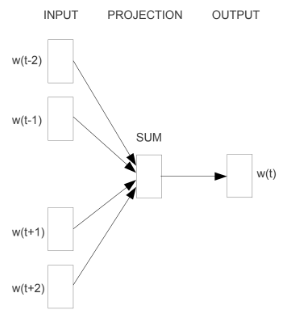
\includegraphics[width=0.6\textwidth]{images/word2vec/cbow.png}
    \caption{Modelo de red de CBOW}
    \label{fig:cbow}
\end{figure}

\subsubsection{\textit{Continuous skip-gram}}

Con el método CBOW, obtenemos las representaciones vectoriales de las palabras a
partir de su contexto. \textit{Skip-gram} se puede considerar como el método
inverso. En este caso, la entrada de la red es la codificación \textit{one-hot}
de la palabra cuya representación se desea obtener, y las salidas son $C$
distribuciones de probabilidad, una para cada palabra del contexto. Este modelo
se puede ver en la Figura \ref{fig:skip-gram} y, comparándolo con el modelo
de CBOW de la Figura \ref{fig:cbow}, observamos que, efectivamente, se trata de
la estructura inversa de este modelo.

\begin{figure}
    \centering
    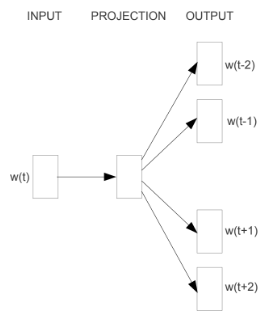
\includegraphics[width=0.5\textwidth]{images/word2vec/skip-gram.png}
    \caption{Modelo de red de \textit{skip-gram}}
    \label{fig:skip-gram}
\end{figure}

\subsection{GloVe}

El nombre de GloVe viene directamente de acortar las palabras \textit{global
    vectors}. Se trata de un algoritmo de aprendizaje no supervisado que trata
de ofrecer un enfoque diferente al de word2vec para la obtención de
representaciones vectoriales de palabras. El problema que los creadores de
GloVe encuentran en word2vec es que, a pesar de que su rendimiento no es
malo, se apoya exclusivamente en la información local del lenguaje, es
decir, en las palabras cercanas a una dada. Por el contrario, GloVe se basa
en las co-ocurrencias de palabras en todo el corpus, una estadística global,
para obtener los vectores de palabras.

En cuanto a su funcionamiento, GloVe no usa redes neuronales, sino que se trata
de un modelo basado en <<conteo>> (\textit{count-based model}). En el algoritmo de
GloVe, se empieza construyendo la matriz de co-ocurrencias del corpus. Para un
vocabulario de $N$ palabras, esta matriz $X$ es de tamaño $NxN$, guardando en
cada celda $X_{ij}$ el número de veces que las palabras $i$ y $j$ aparecen
juntas en el corpus. El algoritmo de GloVe realiza una reducción de la
dimensionalidad de esta matriz, pasando las columnas a ser las características
deseadas, de forma que cada celda $X_{ij}$ contiene el valor de la
característica $j$ para la palabra $i$. Cada palabra se ve entonces representada
por su vector de características.

Realmente, tanto word2vec como GloVe ofrecen resultados similares para tareas de
NLP. La diferencia más importante está en que es muy sencillo paralelizar la
implementación de GloVe, lo que permite entrenar el modelo con más datos de
forma más rápida.

\subsection{\textit{Embedding layer}}
\label{subsec:embedding-layer}

Esta última técnica consiste en añadir al principio de una red neuronal
encargada de realizar alguna tarea de NLP una capa que realice los \textit{word
    embeddings} específicamente. De esta forma, estos \textit{embeddings} se
aprenden de forma conjunta con el modelo de la red.

Las palabras entran a la red usando su codificación \textit{one-hot} y la
\textit{embedding layer} obtiene un vector de dimensión predefinida que
representa a cada una de ellas. Si la red es un perceptrón multicapa, estos
vectores obtenidos se concatenan antes de ser consumidos por el modelo de NLP.
Si, por el contrario, se usa una red neuronal recurrente, se pueden ir enviando
estos vectores de forma secuencial.

El principal problema de esta técnica es que requiere de una gran cantidad de
datos de entrenamiento y puede ser lenta, pero el resultado final es un
\textit{embedding} adaptado a la tarea de NLP específica que se desea realizar
y al texto que se posee.
\newpage
\section{Ejemplo práctico}
\label{sec:example}

Para entender mejor como funcionan los \textit{word embeddings} en las tareas de
NLP, se ha hecho una implementación sencilla en Python con Keras, de la cuál se
muestran en esta sección los fragmentos más
relevantes\footnote{\href{https://colab.research.google.com/drive/18AUH4FhJLhtD1LyWpHcVVL2xvw_n5wN1?usp=sharing}{Cuaderno
        completo}}.

En este ejemplo, se usa el conjunto de datos de noticias de Reuters que
incorpora Keras, que contiene 11228 noticias de 46 categorías diferentes. El
objetivo es entrenar una red neuronal que sea capaz de predecir la categoría de
una noticia en base a su contenido.

Los \textit{word embeddings} se han realizado mediante una capa dedicada al
inicio de la red, tal y como se explicaba en la subsección
\ref{subsec:embedding-layer}. Para esta capa, he realizado dos implementaciones
distintas:

\begin{itemize}
    \item Usando un modelo de GloVe ya entrenado para fijar los pesos.
    \item Entrenando los pesos desde cero.
\end{itemize}

De esta forma, puedo comparar los resultados obtenidos para dos de los
acercamientos más comunes a la hora de trabajar con \textit{embeddings} y que ya
se explicaron en el inicio de la sección \ref{sec:techniques}. El resto de la
red es idéntica en ambos casos.

Para empezar, hay que cargar y preparar los datos. Keras nos proporciona el
conjunto de datos como una lista de secuencias, donde cada secuencia representa
a una noticia y contiene números enteros como IDs de las palabras de dicha
noticia (las palabras como tal no se muestran, pero es irrelevante). Además,
estos IDs están ordenados por ocurrencia en el conjunto entero, de forma que la
palabra con el ID <<1>> es la que más aparece. Al cargar los datos, debemos
indicar con \texttt{num\_words} la cantidad de palabras diferentes que queremos,
seleccionándose siempre las de mayor ocurrencia. En este caso, se han
seleccionado las 20000 palabras más comunes, por lo que en el conjunto de datos
obtenido solo habrá IDs del 0 al 19999. Después, es necesario acotar la longitud
de las secuencias al tamaño deseado con la función \texttt{pad\_sequences}. En
este caso, este tamaño es de 1000 palabras. Por último, se obtiene la
codificación \textit{one-hot} de las etiquetas. Todo esto se puede ver en el
siguiente fragmento de código:

\begin{lstlisting}
from keras.datasets import reuters
from keras.preprocessing.sequence import pad_sequences
from keras.utils import to_categorical
    
(x_train, y_train), (x_test, y_test) = reuters.load_data(num_words=MAX_FEATURES)
word_index = reuters.get_word_index()
    
x_train = pad_sequences(x_train, maxlen=MAX_LEN)
x_test = pad_sequences(x_test, maxlen=MAX_LEN)
    
y_train = to_categorical(y_train, NUM_CLASSES)
y_test = to_categorical(y_test, NUM_CLASSES)
\end{lstlisting}

Ahora, leemos el fichero con el modelo de GloVe pre-entrenado. El modelo elegido
realiza \textit{embeddings} de 100 dimensiones, es decir, las representaciones
vectoriales obtenidas de las palabras tienen 100 dimensiones. En el siguiente
fragmento de código se lee este modelo del fichero y se guardan los
\textit{embeddings} de cada palabra en un mapa \texttt{embeddings\_index} como
\textit{arrays}.

\begin{lstlisting}
import os
import numpy as np
    
embeddings_index = {}
f = open(os.path.join('.', 'glove.6B.100d.txt'))
for line in f:
    values = line.split()
    word = values[0]
    coefs = np.asarray(values[1:], dtype='float32')
    embeddings_index[word] = coefs
f.close()
\end{lstlisting}

Ahora, se debe usar este \texttt{embeddings\_index} para construir una matriz
que se le pueda asignar a la capa de \textit{embedding} de la red. Para ello, se
recorre el índice de palabras \texttt{word\_index} del conjunto de datos
obtenido de Keras y se comprueba si existen dichas palabras en el
\texttt{embeddings\_index} (recordar que se trabaja con IDs numéricos, no con
las palabras reales). En caso afirmativo, se copia el \textit{array} con el
\textit{embedding} de la palabra a su fila correspondiente en la matriz,
si no, se rellena esa fila con ceros.

\begin{lstlisting}
embedding_matrix = np.zeros((len(word_index) + 1, EMBEDDING_DIM))
for word, i in word_index.items():
    embedding_vector = embeddings_index.get(word)
    if embedding_vector is not None:
        # words not found in embedding index will be all-zeros.
        embedding_matrix[i] = embedding_vector
\end{lstlisting}

Una vez hecho esto, ya podemos construir la red inicializando los pesos de la capa
de \textit{embedding} con la matriz construida e indicando que esta capa no se
entrena (\texttt{trainable=False}), haciendo que sea fija. El resto de la red es
una red convolucional sencilla con salida \textit{softmax}. Después de entrenar
durante 5 épocas, conseguimos un \textit{accuracy} de 0.66 sobre el conjunto de
prueba, bastante bajo.

\begin{lstlisting}
from keras.models import Sequential
from keras.layers import Embedding, Conv1D, MaxPooling1D, Flatten, Dense, Dropout
from keras.losses import categorical_crossentropy
    
fixed_model = Sequential()
fixed_model.add(Embedding(len(word_index) + 1,
                        EMBEDDING_DIM,
                        weights=[embedding_matrix],
                        input_length=MAX_LEN,
                        trainable=False))
fixed_model.add(Conv1D(128, 5, activation='relu'))
fixed_model.add(MaxPooling1D(5))
fixed_model.add(Conv1D(128, 5, activation='relu'))
fixed_model.add(MaxPooling1D(5))
fixed_model.add(Conv1D(128, 5, activation='relu'))
fixed_model.add(MaxPooling1D(35))
fixed_model.add(Flatten())
fixed_model.add(Dense(128, activation='relu'))
fixed_model.add(Dense(NUM_CLASSES, activation='softmax'))
    
fixed_model.compile(loss=categorical_crossentropy,
                    optimizer='adam',
                    metrics=['accuracy'])

fixed_model.fit(x_train, y_train,
                validation_split=0.1,
                epochs=5,
                batch_size=32)
\end{lstlisting}

Probamos ahora a entrenar una capa de \textit{embedding} desde cero. Como se
puede ver en el siguiente fragmento de código, la definición de la red es
idéntica excepto que no se predefine una matriz de pesos para la capa de
\textit{embedding}. Entrenamos esta red durante 5 épocas también y el modelo
resultante obtiene 0.72 de \textit{accuracy} sobre el conjunto de prueba.

\begin{lstlisting}
trained_model = Sequential()
trained_model.add(Embedding(len(word_index) + 1,
                            EMBEDDING_DIM,
                            input_length=MAX_LEN))
trained_model.add(Conv1D(128, 5, activation='relu'))
trained_model.add(MaxPooling1D(5))
trained_model.add(Conv1D(128, 5, activation='relu'))
trained_model.add(MaxPooling1D(5))
trained_model.add(Conv1D(128, 5, activation='relu'))
trained_model.add(MaxPooling1D(35))
trained_model.add(Flatten())
trained_model.add(Dense(128, activation='relu'))
trained_model.add(Dense(NUM_CLASSES, activation='softmax'))
    
trained_model.compile(loss=categorical_crossentropy,
                    optimizer='adam',
                    metrics=['accuracy'])

trained_model.fit(x_train, y_train,
                validation_split=0.1,
                epochs=5,
                batch_size=32)
\end{lstlisting}

El hecho de que el resultado haya sido mejor para la capa de \textit{embedding}
entrenada que para la predefinida no indica que se trate de una acercamiento más
correcto, sino que es mejor para este ejemplo concreto.
\newpage

\bibliographystyle{ieeetr}
\bibliography{sources}
\end{document}
